\setlength{\arrayrulewidth}{.5mm}
\setlength{\tabcolsep}{5pt}
\renewcommand{\arraystretch}{2}

\subsection{Introduzione}
Il team seguirà la metodologia di progetto RUP, in seguito sono specificati il piano di progetto e le
iterazioni che lo compongono.

\subsection{Piano}
Il piano di progetto si suddivide in 4 fasi temporali:
\begin{itemize}
    \item Inception
    \item Elaboration
    \item Construction
    \item Transition
\end{itemize}
Le attività coinvolte sono le seguenti:
\begin{itemize}
    \item Studio di fattibilità
    \item Raccolta dei requisiti
    \item Analisi e progetto
    \item Implementazione
    \item Test
\end{itemize}
Le varie attività si distribuiranno nelle fasi temporali in maniera eterogenea, in relazione a quanto una particolare attività è significativa in una certa fase. Qui sotto è raffigurato il processo in un grafico descrittivo: \vspace{0.6cm}

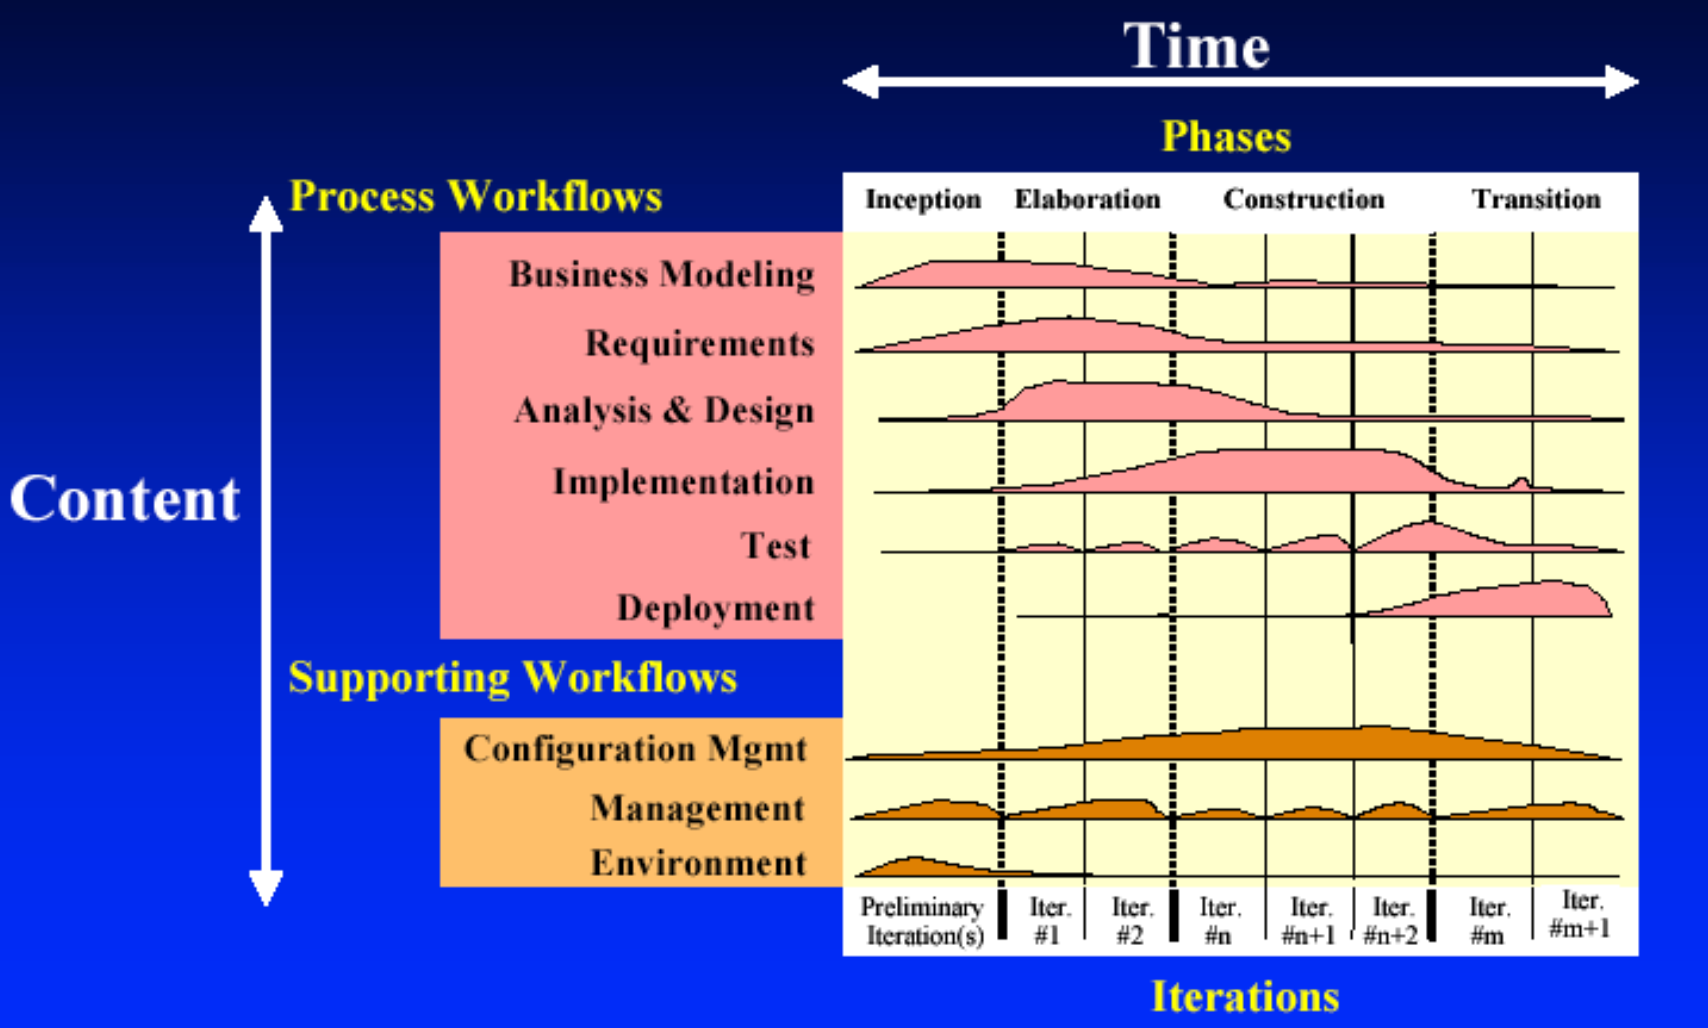
\includegraphics[width=12cm]{images/RUPplan.png}

\subsection{Iterazioni}

\begin{center}

\begin{tabular}{ |p{2cm}|p{10cm}|  }
\hline
Nome & Iterazione 1 \\\hline
Fase & Inception \\\hline
Inizio & 20/11/2019 \\\hline
Fine &  1/12/2019 \\\hline
Obbiettivi & 
	\begin{compactitem}
		\item Analisi del problema e prima stesura del documento di Visione
		\item Definire configurazione iniziale del sistema
		\item Analizzare la fattibilità del progetto, dal punto di vista tecnico ed economico
		\item Formulazione di una prima proposta di Contratto
		\item Formulazione documento Glossario
	\end{compactitem}\\\hline
Stato &  Conclusa \\\hline
\end{tabular}
\label{table:1}\newline

\begin{tabular}{ |p{2cm}|p{10cm}|  }
\hline
Nome & Iterazione 2 \\\hline
Fase & Inception \\\hline
Inizio & 15/12/2019 \\\hline
Fine &  18/12/2019 \\\hline
Obbiettivi & 
	\begin{compactitem}
		\item Stesura del piano di progetto
		\item Revisione e aggiornamento della proposta di contratto
		%\item Aggiornamento del Glossario
	\end{compactitem}\\\hline
Stato &  Conclusa \\\hline
\end{tabular}
\label{table:2}\newline

\begin{tabular}{ |p{2cm}|p{10cm}|  }
\hline
Nome & Iterazione 3 \\\hline
Fase & Inception \\\hline
Inizio & 01/02/2020 \\\hline
Fine &  14/02/2020 \\\hline
Obbiettivi & 
	\begin{compactitem}
		%\item Analisi dei requisiti e stesura del relativo documento di Specifica
		%\item Analisi e gestione dei rischi e stesura del relativo documento
		
		\item Individuare tutti i requisiti funzionali con priorità primaria
		\item Individuare almeno il 50\% dei requisiti funzionali con priorità secondaria
		\item Individuare almeno il 50\% dei requisiti non funzionali
		\item Descrivere ad alto livello i requisiti individuati
		\item Individuare almeno il 70\% dei rischi e stendere un piano di gestione per ciascun rischio
		\item Aggiornamento del Glossario
	\end{compactitem}\\\hline
Stato &  Conclusa \\\hline % Svolgimento 
\end{tabular}
\label{table:3}\newline

\begin{tabular}{ |p{2cm}|p{10cm}|  }
\hline
Nome & Milestone 1\\\hline
Fase & Inception \\\hline
Inizio & 17/02/2020 \\\hline
Fine &  17/02/2020 \\\hline
Obbiettivi & 
	\begin{compactitem}
		\item I requisiti primari sono stati individuati e descritti correttamente
		\item Almeno il 70\% dei rischi è stato individuato ed è stato creato un piano di gestione per ciascun rischio
		\item Tutte le iterazioni sono state programmate
	\end{compactitem}\\\hline
Stato &  Raggiunta \\\hline
\end{tabular}
\label{table:milestone1}\newline

\begin{tabular}{ |p{2cm}|p{10cm}|  }
\hline
Nome & Iterazione 4 \\\hline
Fase & Elaboration \\\hline
Inizio & 17/02/2020 \\\hline
Fine &  24/02/2020 \\\hline
Obbiettivi & 
	\begin{compactitem}
		\item Definire un modello dettagliato dei casi d'uso (relativo ai requisiti funzionali primari, e al primo 50\% dei requisiti funzionali secondari individuati) 
		\item Individuare il restante 50\% dei requisiti funzionali secondari
		\item Individuare il restante 50\% dei requisiti non funzionali
		\item Individuare un ulteriore 15\% dei rischi  e stendere un piano di gestione per ciascun rischio
	\end{compactitem}\\\hline
Stato &  Conclusa \\\hline
\end{tabular}
\label{table:4}\newline

\begin{tabular}{ |p{2cm}|p{10cm}|  }
\hline
Nome & Iterazione 5 \\\hline
Fase & Elaboration \\\hline
Inizio & 26/02/2020 \\\hline
Fine &  03/03/2020  \\\hline
Obbiettivi & 
	\begin{compactitem}
		%\item Raffinamento dei documenti Glossario, Requisiti
		%\item Definire i diagrammi UML dei vari casi d'uso
		%\item Creazione di una matrice di tracciabilità
		\item Definire un modello dettagliato dei casi d'uso (relativo al restante 50\% dei requisiti funzionali secondari)
		\item Individuare il restante 15\% dei rischi  e stendere un piano di gestione per ciascun rischio
		\item Effettuare una stima dei costi 
	\end{compactitem}\\\hline
Stato &  Svolgimento \\\hline
\end{tabular}
\label{table:5}\newline

\begin{tabular}{ |p{2cm}|p{10cm}|  }
\hline
Nome & Iterazione 6 \\\hline
Fase & Elaboration \\\hline
Inizio & 05/03/2020 \\\hline
Fine &  14/03/2020  \\\hline
Obbiettivi & 
	\begin{compactitem}
		%\item Individuare le classi e le componenti per realizzare il sistema (per tutti i casi d'uso a priorità più alta, e facendo riferimento ai requisiti non funzionali)
		%\item Modellare l'architettura del sistema
		\item Analisi del sistema (individuare classi e componenti per la realizzazione del sistema, e descrivere le loro interazioni)
		%definire comportamento dell'architettura rispetto alle esigenze individuate
		%\item Creazione schede CRC
		%\item Creazione diagramma EBC
		%\item Creazione diagrammi di sequenza
		%\item Creazione diagrammi di classi
	\end{compactitem}\\\hline
Stato &  Programmata \\\hline
\end{tabular}
\label{table:6}\newline

\begin{tabular}{ |p{2cm}|p{10cm}|  }
\hline
Nome & Iterazione 7 \\\hline
Fase & Elaboration \\\hline
Inizio & 15/03/2020 \\\hline
Fine & 25/03/2020 \\\hline
Obbiettivi & 
	\begin{compactitem}
		%\item Raffinamento e revisione dei vari diagrammi definiti durante l'iterazione 6
		\item Design del sistema (relativo agli use case primari)
		\item Realizzazione dei test relativi al 20\% degli use case
	\end{compactitem}\\\hline
Stato &  Programmata \\\hline
\end{tabular}
\label{table:7}\newline

\begin{tabular}{ |p{2cm}|p{10cm}|  }
\hline
Nome & Milestone 2\\\hline
Fase & Elaboration \\\hline
Inizio & 26/03/2020 \\\hline
Fine &  26/03/2020 \\\hline
Obbiettivi & 
	\begin{compactitem}
		\item Tutti i rischi sono stati individuati ed è stato creato un piano di gestione per ciascun rischio
		\item \'E stata effettuata una stima dei costi attendibile
		\item Prendere una decisione Go/NoGo
		\item \'E stata effettuata un'analisi del sistema coerente con i requisiti (sia funzionali che non funzionali)
	\end{compactitem}\\\hline
Stato &  Programmata \\\hline
\end{tabular}
\label{table:milestone3}\newline

\begin{tabular}{ |p{2cm}|p{10cm}|  }
\hline
Nome & Iterazione 8 \\\hline
Fase & Construction \\\hline
Inizio & 27/03/2020 \\\hline
Fine &  04/04/2020  \\\hline
Obbiettivi & 
	\begin{compactitem}
		%\item Creazione di un diagramma architetturale dell'intero sistema
		\item Completamento design del sistema
		\item Realizzazione del restante 80\% dei test
	\end{compactitem}\\\hline
Stato &  Programmata \\\hline
\end{tabular}
\label{table:8}\newline

\begin{tabular}{ |p{2cm}|p{10cm}|  }
\hline
Nome & Milestone 3\\\hline
Fase & Construction \\\hline
Inizio & 05/04/2020 \\\hline
Fine &  05/04/2020 \\\hline
Obbiettivi & 
	\begin{compactitem}
		\item Il sistema rispetta tutti i requisiti definiti nella fase di analisi (sia funzionali che non funzionali)
		\item Sono stati definiti test per ogni funzionalità del sistema
		\item Il sistema ha superato tutti i test definiti in precedenza
	\end{compactitem}\\\hline
Stato &  Programmata \\\hline
\end{tabular}
\label{table:milestone4}\newline

\begin{tabular}{ |p{2cm}|p{10cm}|  }
\hline
Nome & Iterazione 9 \\\hline
Fase & Transition \\\hline
Inizio & 06/04/2020 \\\hline
Fine &  10/04/2020  \\\hline
Obbiettivi & 
	\begin{compactitem}
		\item Raccolta Feedback di utilizzo degli utenti
		\item Creazione degli ultimi test basati sul feedback degli utenti
		\item Creare una release finale
	\end{compactitem}\\\hline
Stato &  Programmata \\\hline
\end{tabular}
\label{table:9}\newline

\begin{tabular}{ |p{2cm}|p{10cm}|  }
\hline
Nome & Milestone 4\\\hline
Fase & Construction \\\hline
Inizio & 10/04/2020 \\\hline
Fine &  10/04/2020 \\\hline
Obbiettivi & 
	\begin{compactitem}
		\item Release finale creata
	\end{compactitem}\\\hline
Stato &  Programmata \\\hline
\end{tabular}
\label{table:milestone5}\newline


\end{center}

\subsection{Diagramma di Gantt}
\vspace{0.5cm}
\begin{center}
	\hspace*{-2cm}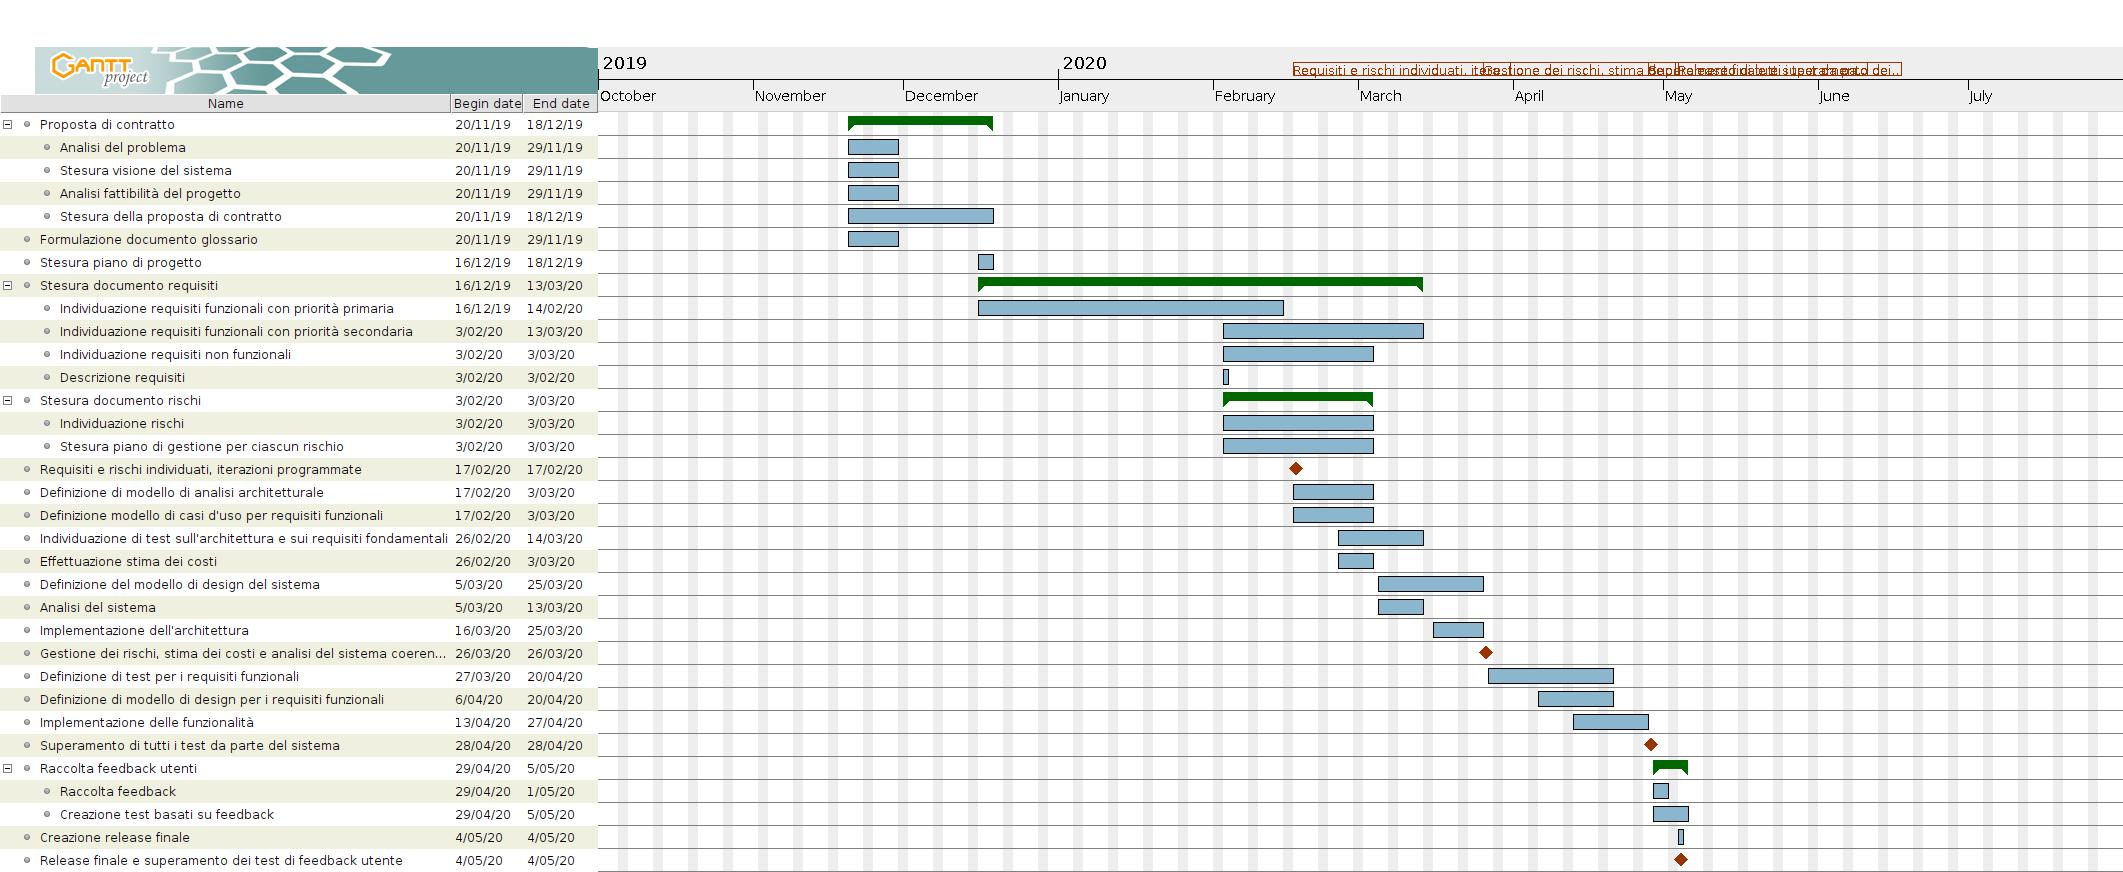
\includegraphics[width=16cm]{Gantt_NexiFy.jpg}
\end{center}
\vspace{2cm}

\clearpage
\noindent{\LARGE \textbf{Revisioni 4-5}} \\ \\
\begin{tabular}{|c | c | c | c|} 
 	\hline
	 Numero & Data & Descrizione \\ [0.5ex] 
	\hline\hline
	1 & 17/12/2019 & Stesura iniziale \\ 
	\hline
	2 & 16/02/2020 & \thead{Specificati meglio gli obiettivi da raggiungere per ogni iterazione,\\e non gli strumenti usati per raggiungerli} \\ 
	\hline
	3 & 26/02/2020 & Revisione del contratto e del piano di progetto \\ 
	\hline
\end{tabular}